\documentclass[10pt]{article}
\usepackage[utf8]{inputenc}
\usepackage{graphicx}
\usepackage{url}
\usepackage{color}
\usepackage{amsmath}
\usepackage{pgf}
\usepackage{hyperref}
\usepackage{float}


\newtheorem{question}{Question}

\setlength {\parskip}{2mm}
\setlength {\parindent}{0mm}
\addtolength{\topmargin}{-2.5cm}
\addtolength{\textheight}{4cm}
\addtolength{\evensidemargin}{-20mm}
\addtolength{\oddsidemargin}{-20mm}
\addtolength{\textwidth}{40mm}
\thispagestyle{empty}
\pagestyle{empty}
\usepackage{graphicx}


\begin{document}

{\flushright \small \tt Master Bioinformatique parcours MISO 2022-23}

\begin{center}
\textbf{M\'ethodes pour l'Analyse Bioinformatique des S\'equences}

\end{center}


\hrule

\bigskip

\begin{center}

\textbf{\Large Projet 1: structure secondaire des ARN}    
\end{center}

\bigskip

Les ARN sont des mol\'ecules simple brin dont la fonction est li\'ee \`a plusieurs niveaux d’information: la s\'equence form\'ee de l’enchainement des nucl\'eotides A, C, G et U, la structure secondaire qui capture les appariements entre nucl\'eotides, l’organisation de la structure dans l’espace, et enfin les interactions avec les autres mol\'ecules pr\'esentes dans la cellule. Parmi ces diff\'erents niveaux, la structure secondaire est d\'eterminante, car elle constitue un \'echaffaudage pour le repliement final.

Les appariements de la structure secondaire sont de trois sortes:
\begin{itemize}
\item C avec G, impliquant 3 liaisons hydrogène
\item  A avec U, impliquant 2 liaisons hydrogène
\item G avec U, impliquant 1 liaison hydrogène
\end{itemize}

Ces appariements ont également la propriété de ne pas se croiser, et de ne pas se former entre nucléotides dont la distance sur la séquence est inférieure à trois. Toute position est impliquée dans \emph{au plus} une paire de bases.  Voir l'exemple de la Figure \ref{fig:arn}.

L'objectif du projet est de créer une librairie qui permet de manipuler des structures secondaires d'ARN. Un exemple de librairie est représentée au format UML Figure \ref{fig:uml}.

Vous implémenterez cette librairie dans un script python, afin de répondre aux différentes questions du projet.



\section*{Partie 1: formats de description}

Il existe deux formats principaux pour décrire les structures secondaires: le format CT (connect) et le format parenthésé. 

Le format CT est un format tabulé constitué de trois colonnes, avec $n$ lignes où $n$ est la longueur de la séquence d'ARN. La première colonne indique la position du nucléotide dans la séquence (de 1 à $n$), la deuxième colonne indique la valeur du nucléotide à cette position (A, C, G ou U) et la troisième colonne indique avec quelle position le nucléotide est apparié. Dans le cas où le nucléotide n'est pas apparié (il est libre),  on indique 0 par convention. Les appariements sont donc représentés par des couples de positions. Un exemple est donné en Figure \ref{fig:CT}.

Le format parenthésé ressemble au format Fasta, avec une ligne supplémentaire pour les appariements. La première ligne est donc une ligne d'entête commençant par un chevron $>$. La deuxième ligne contient la séquence nucléotidique. La troisième ligne indique les appariements deux à deux sous forme de parenthèses: la parenthèse ouvrante est le premier nucléotide de l'appariement et la parenthèse fermante correspondante le second nucléotide de l'appariement. Les positions libres sont indiquées avec des points. Un exemple est donné en Figure \ref{fig:parenthese}.

\begin{figure}
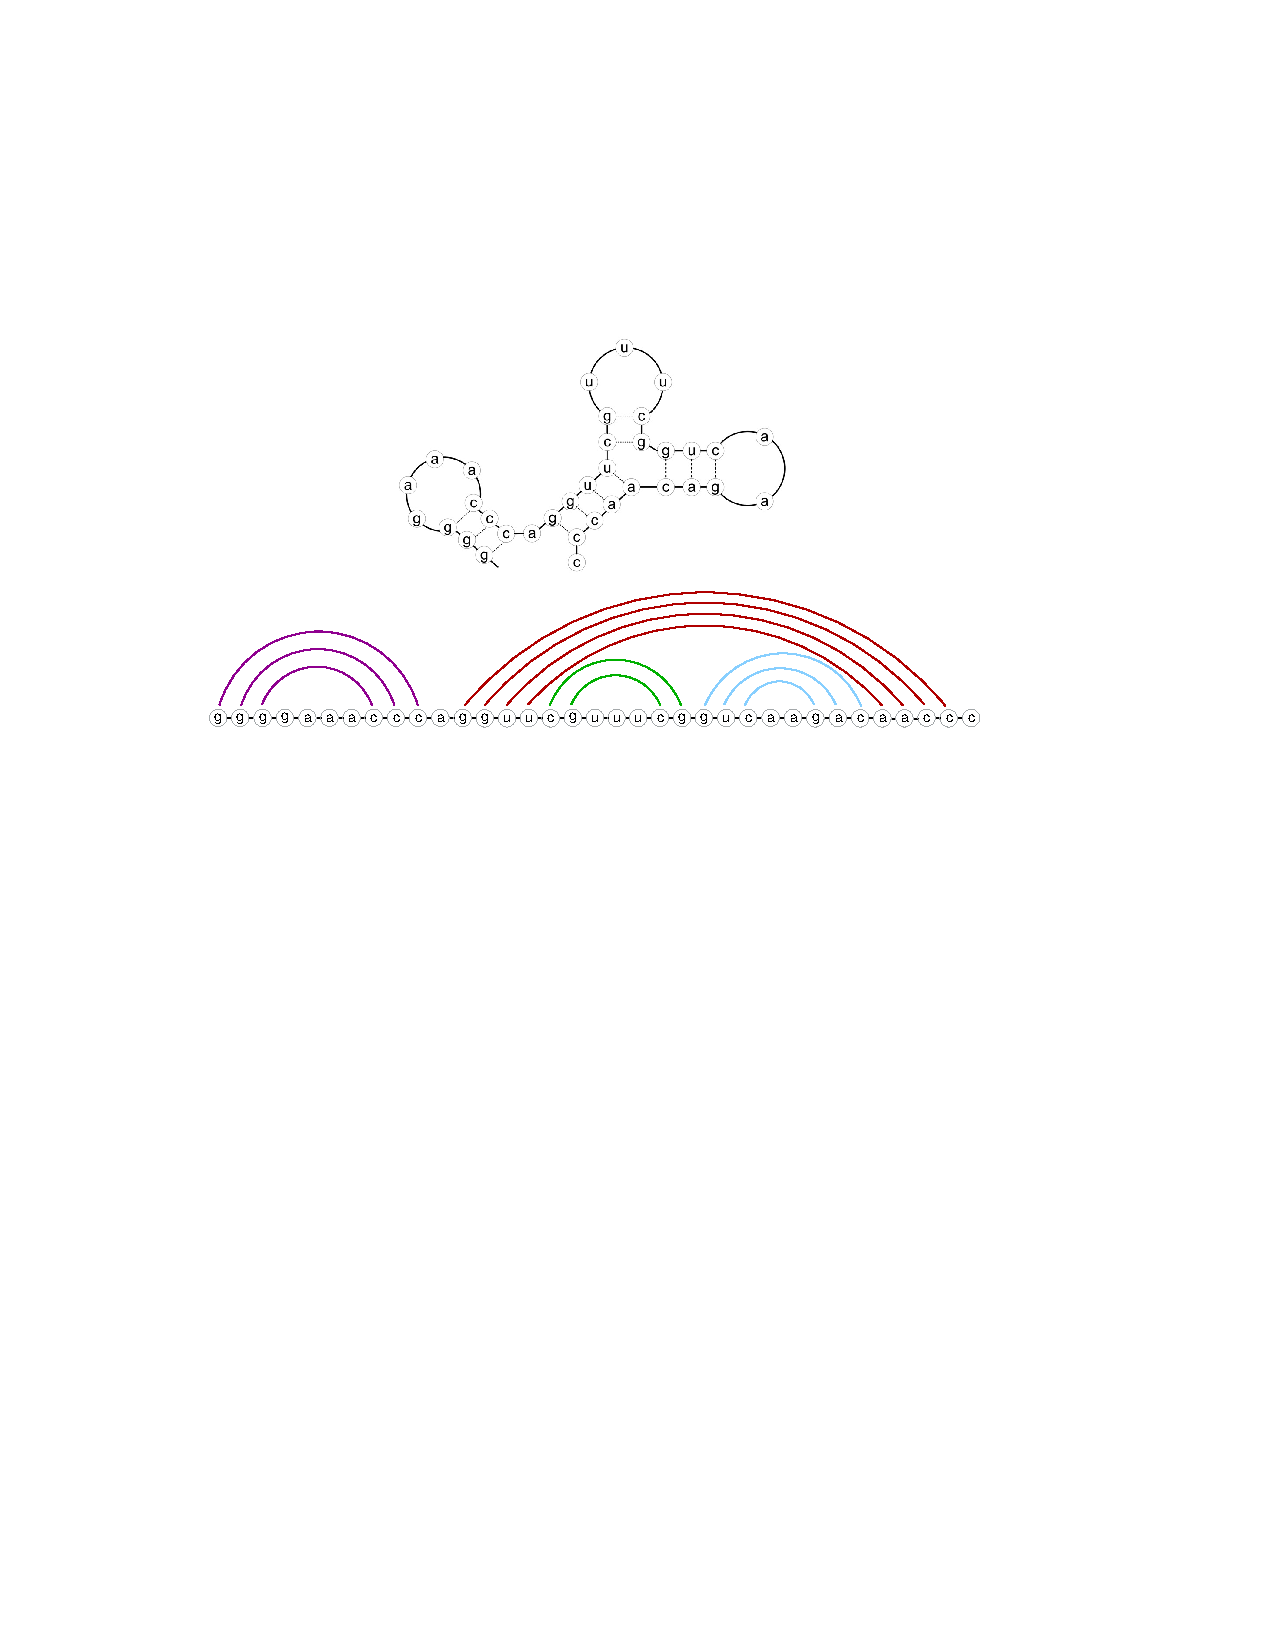
\includegraphics[width=\textwidth]{structure_secondaire_ARN.pdf}
\caption{Exemple de structure secondaire}
\label{fig:arn}
\end{figure}

\begin{figure}
\begin{verbatim}
1  g 10
2  g 9
3  g 8
4  g 0
5  a 0
6  a 0
7  a 0
8  c 3
9  c 2
10 c 1
11 a 0
12 g 34
13 g 33
14 u 32
15 u 31
16 c 22
17 g 21
18 u 0
19 u 0
20 u 0
21 c 17
22 g 16
23 g 30
24 u 29
25 c 28
26 a 0
27 a 0
28 g 25
29 a 24
30 c 23
31 a 15
32 a 14
33 c 13
34 c 12
35 c 0
\end{verbatim}
\caption{Représentation au format CT de la structure de la Figure \ref{fig:arn}}
\label{fig:CT}
\end{figure}

\begin{figure}
\large
\begin{verbatim}
>sequence test
ggggaaacccagguucguuucggucaagacaaccc
(((....))).((((((...))(((..))))))).
\end{verbatim}
\caption{Représentation au format parenthésée de la structure de la Figure \ref{fig:arn}}
\label{fig:parenthese}
\end{figure}


\begin{question}
  Parser une structure d'ARN au format Connect, vérifier sa validité et calculer le nombre total de liaisons hydrogènes de la structure. 
\end{question}

\begin{question}
  Parser une structure d'ARN au format parenthésé, vérifier sa validité et calculer le nombre total de liaisons hydrogènes de la structure.
  \end{question}

  \section*{Partie 2: équivalence de deux structures secondaires}

  Une structure secondaire peut être décomposée en {\em tiges}: une tige est une succession d'appariements consécutifs. Par exemple, la structure de la Figure 1 contient quatre tiges, en violet, rouge, vert et bleu. On dit que deux structures sont {\em équivalentes} si elles contiennent la même organisation en tiges. tiges.

  \begin{question}
Ecrire une fonction qui détermine si deux structures sont équivalentes
    \end{question}


 \section*{Partie 3: prédiction de structure}

 La prédiction de structure consiste à déterminer l'ensemble des appariements à partir de la séquence nucléoditique. Pour cela, on calcule la structure qui maximise le nombre de liaisons hydrogène, ce qui se fait par programmation dynamique.
  
 \begin{question}
   Ecrire une fonction qui prend en entrée une séquence d'ARN et calcule le nombre
   de liaisons hydrogènes maximal.
  \end{question}

\begin{question}
  Compléter la question précédente en reconstruisant la structure optimale (ou une structure optimale s'il en existe plusieurs).
\end{question}


\begin{question}(falcultative)
Ecrire une fonction qui calcule toutes les structures optimales possibles.
\end{question}

\begin{figure}
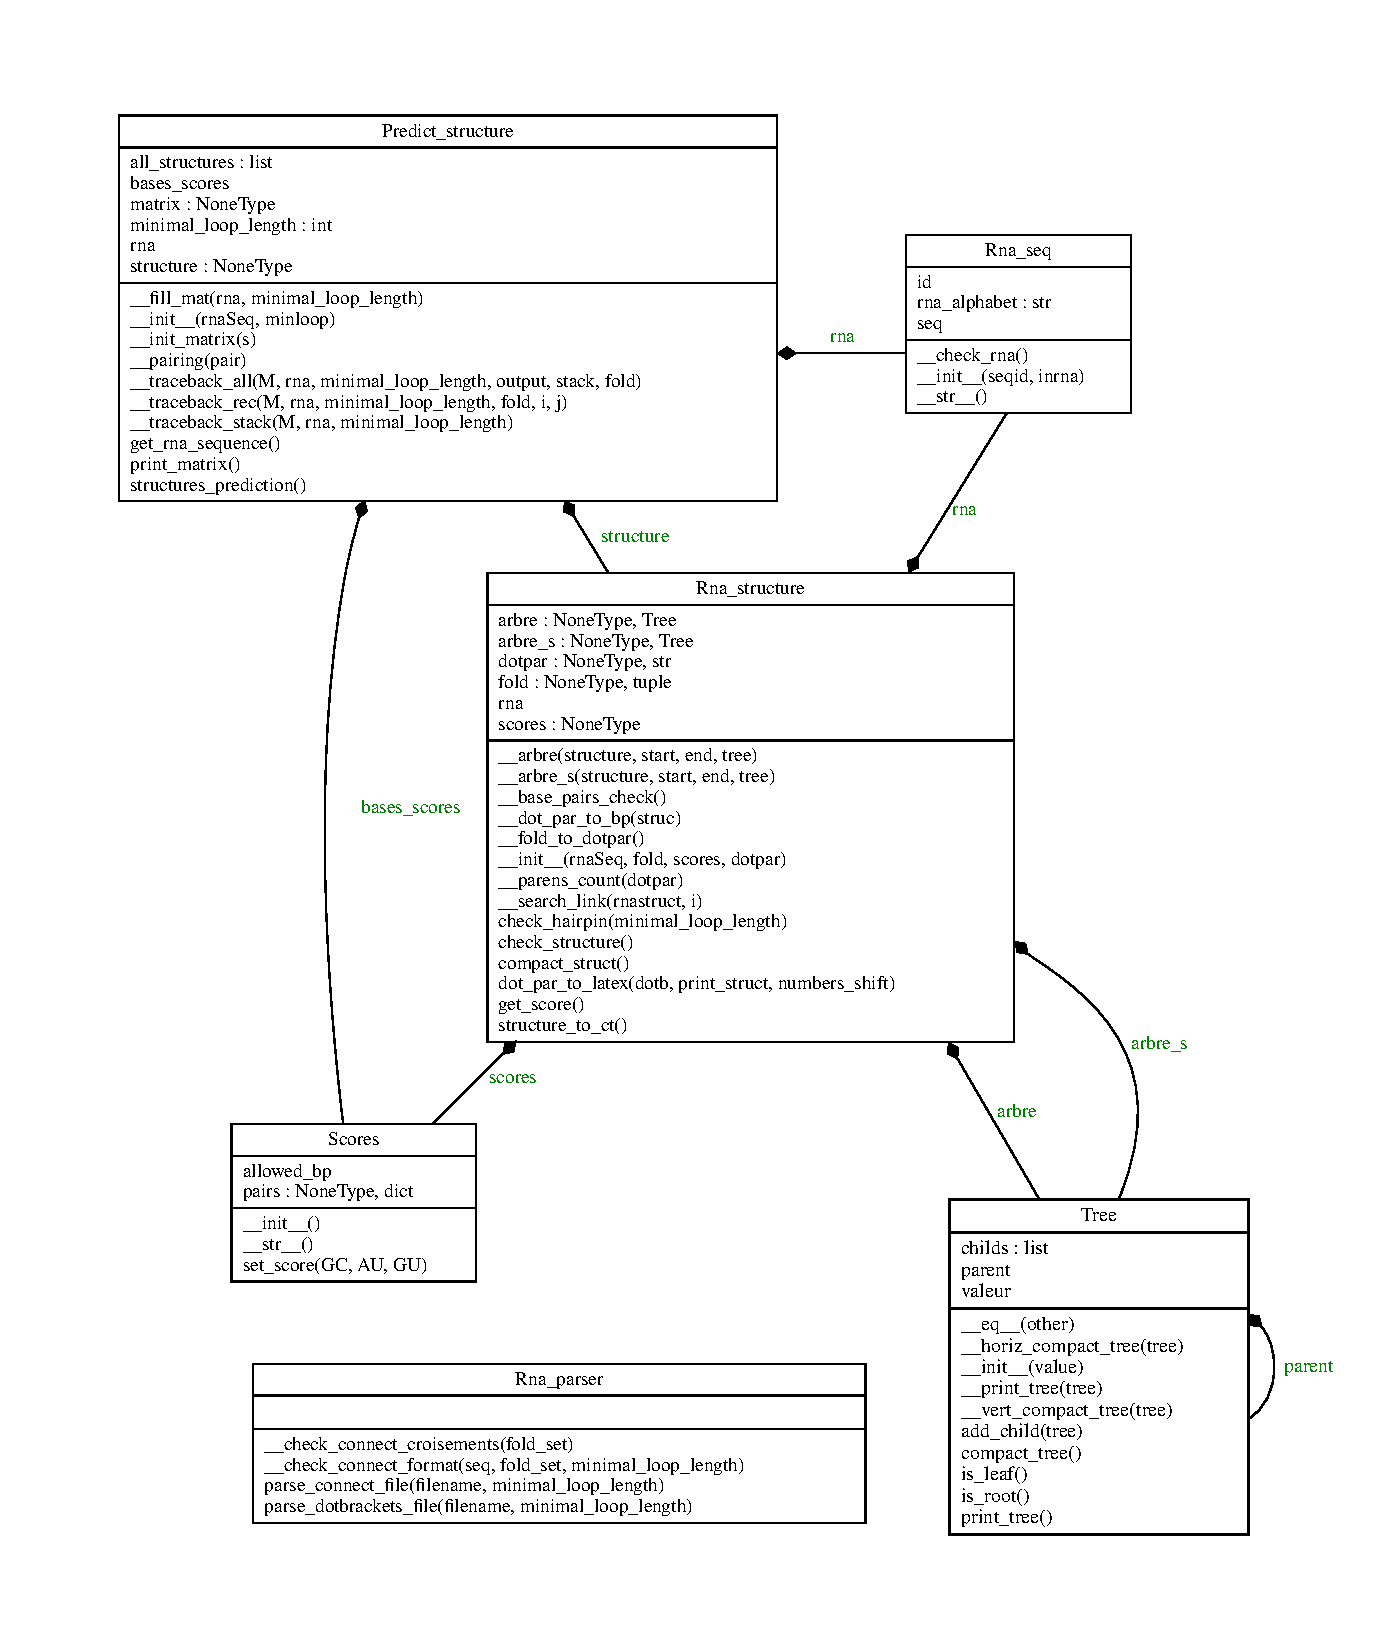
\includegraphics[width=\textwidth]{Rnalib.pdf}
\caption{Exemple d'un diagramme UML pour la librairie}
\label{fig:uml}
\end{figure}

\end{document}